\chapter{Architectures}

Overall, we developed six different architectures, each one having from two to three different variations depending on the way the \textit{Divine Comedy} was tokenized, for a total of 13 models.
In this chapter we will briefly explain the characteristic of each architecture, but first we must say something about the general aspects that will recur for all of them.

\subsubsection{\textsc{Text Prcoessing}}

First of all, the \texttt{mark} function inside the \texttt{text\_processing.markers} module was developed to insert some special markers in the original \textit{Divine Comedy}.
Together with that, we developed its complementary function \texttt{unmark}, used to get a cleaned text from the ones generated by the Neural Networks.

These markers were intended to give some structure to the text in order to make it easier for the Neural Network to understand the tokenized text. More specifically, the markers are \texttt{"=startofcantica="}, \texttt{"=endofcantica="}, \texttt{"=startofcanto="} \texttt{"=endofcanto="} and \texttt{"tercet"}.

Here is an example of a sample of text before and after the marking:

\begin{paracol}{2}
\scriptsize{\begin{verbatim}
INFERNO

- Canto I

Nel mezzo del cammin di nostra vita
mi ritrovai per una selva oscura,
ché la diritta via era smarrita.

Ahi quanto a dir qual era è cosa dura
esta selva selvaggia e aspra e forte
che nel pensier rinova la paura!
\end{verbatim}}
\switchcolumn
\scriptsize{\begin{verbatim}


=startofcantica=
=startofcanto=
Nel mezzo del cammin di nostra vita
mi ritrovai per una selva oscura,
ché la diritta via era smarrita.
=tercet=
Ahi quanto a dir qual era è cosa dura
esta selva selvaggia e aspra e forte
che nel pensier rinova la paura!
\end{verbatim}}
\end{paracol}


\subsubsection{\textsc{Text Tokenization}}

The tokenization of the text took advantage of Tensorflow Dataset tokenizers, which can be found in the package \texttt{tfds.features.text}.
For our purposes, we built up three of them (a \texttt{char\_tokenizer}, a \texttt{word\_tokenizer} and a \texttt{subword\_tokenizer}), each of which can be found in the package \texttt{text\_processing.tokenizers} of our repository, and is responsible to take care not only of alphanumeric symbols but also of punctuation symbols, newline symbols, white spaces and special markers, all separate tokens that are independently learnt and generated by the Neural Networks.

Each of the six architectures have been tested with both a \textit{Word-Level} and \textit{Subword-Level} tokenization, and for the first architecture we also tried a \textit{Char-Level} implementation.
At the end of the day, the \textit{Subword-Level} tokenization was the one giving best results.
In fact, as the tokenizer was fed with the \textit{Divine Comedy} and it has the ability to split the words into the most frequent subwords, the text could be tokenized in something that vaguely resembled syllables, giving, both from a theoretical and a practical point of view, a great insight to the Neural Network when considering verse structure and rhyming scheme. 

Here is an example of the subword tokenization of a sample of text:

\begin{paracol}{2}
\scriptsize{\begin{verbatim}
    =startofcantica=
    =startofcanto=
    Nel mezzo del cammin di nostra vita
    mi ritrovai per una selva oscura,
    ché la diritta via era smarrita.
    =tercet=
\end{verbatim}}
\switchcolumn
\scriptsize{\begin{verbatim}
    =startofcantica=
    =startofcanto=
    Nel mez zo del cam min di nos tra vit a
    mi rit rov ai per una sel va osc ura ,
    ché la dir itt a via era sma rri ta .
    =tercet=
\end{verbatim}}
\end{paracol}

\subsubsection{\textsc{Hyperparameters and Results}}

All the tested models had their own hyperparameters, which could be related not only to the actual architecture of the Neural Network but also to the construction of the dataset.
In this last case, the hyperparameters were the same for all the models, namely:
\begin{itemize}
    \item the window size to extract the input strings, or rather the sequence length
    \item the number of tokens to skip from one window to the following one, or rather the step length
    \item the train/validation splitting percentage
    \item the size of the batch
    \item the number of training epochs
\end{itemize}

Generally, these parameters can be inferred (e.g. for the sequence length we chose the minimum amount of tokens necessary to get at least the previous three verses entirely) or have a minor influence on the final results, thus, during our experiments to find the best set of hyperparameters, we mainly focused on the hyperparameters of the network.
In any case, we automated the process in order to test the performances of each configuration/model, varying the temperature factor of the generation as well, and stored a summary of the results for each test into a series of \texttt{.txt} files placed in the \texttt{results} folder of the repository.

\subsubsection{\textsc{Optimizer and Loss Function}}

Each model was compiled with either the default or a custom \texttt{Adam} optimizer, where the latter case is referred to the \textit{Transformer} model, whose specifications for a better optimizer were given in the original paper \parencite{vaswani2017attention}.

Instead, as loss function we always used the \texttt{Sparse Categorical Crossentropy} except that for the last model, the \textit{GAN}, that obviously used the \texttt{Binary Crossentropy} of the discriminator to perform backpropagation both during the discriminator and the adversarial training.

\section{Plain RNN}

As many models for text generation (and other \textit{Natural Language Processing} tasks as well) have been proposed all over the years, we decided to keep our first model as simple as possible to set a sort of lower bound that would have been useful for the successive architectures.

\begin{figure}[!htb]
    \centering
    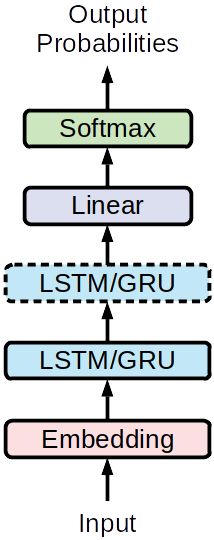
\includegraphics[scale=0.65]{images/model-1.png}%
    \caption{Plain RNN Architecture}%
    \label{plain-rnn}
\end{figure}

Therefore, inspired by Karpathy's work \parencite{karpathy2015unreasonable}, universally recognized as a milestone in the field of \textit{Natural Language Processing}, we developed the model in figure \ref{plain-rnn} consisting of an initial \textsc{Embedding} layer, mapping the tokenized input into a dense vector, which is then passed to either one or two \textsc{RNN} layer(s) and, eventually, to a final \textsc{Dense} layer, post-processed using softmax activation in order to output the probability of each token.
Given that standard \textsc{RNN} layers notoriously suffer from the so-called vanishing gradient problem, which arises in the backpropagation step, we decided to use either \textsc{LSTM} (\textsc{Long Short-Term Memory}) layers \parencite{hochreiter1997long} or \textsc{GRU} (\textsc{Gated Recurrent Units}) layers \parencite{chung2014empirical}, two special kinds of \textsc{RNN} layers developed to overcome this known problem.

Finally, as we said during the introduction of this chapter, the input and output samples we used had a fixed length, the so-called \texttt{sequence length}.
One important thing to notice is that we did not use a long sample as input and just a single token as output, but the output was instead the exact input sequence shifted by one token\footnote{
    If the input sequence is made up of the ordered set of tokens $$\{i, ..., i + sequence length - 1\}$$ taken from the \textit{Divine Comedy}, then the output is made up of the ordered set of tokens $$\{i + 1, ..., i + sequence length\}$$
}, so that the network could understand the inner patterns of the text as well.

\subsubsection{\textsc{Hyperparameters and Results}}

As we said in the introductory part of this chapter, we instantiated this architecture in three different variations, depending on the way the input text was tokenized, namely a \textit{Char-Level} model, a \textit{Word-Level} model and a \textit{Subword-Level} model.

Each of these variations had the same, independent set of hyperparameters, which we tried to tune by testing different values.
They are:
\begin{itemize}
    \item The dimension of the \textsc{Embedding} layer
    \item The kind of \textsc{RNN} (\textsc{GRU} or \textsc{LSTM})
    \item The number of \textsc{RNN} layers (either one or two), and their respective number of units
    \item The dropout rate of the \textsc{RNN} layers
\end{itemize}

After all, even though being very basic, these models were able to produce discrete results.
Taking into consideration only the configurations scoring high the \texttt{n-grams plagiarism} metric, i.e. considering only the generated samples that were not simply a copy-paste of the original \textit{Divine Comedy}, with each of the three variations we could achieve great scores (up to \textit{0.99}) in terms of \texttt{structuredness}, showing that, at least, the network had been able to understand where and how to split one tercet from the other.

As regards the structure of the verses, instead, we could achieve almost optimal results mainly with the \textit{Char-Level} and the \textit{Subword-Level} models.
In fact, while these two models were able to generate samples scoring up to \textit{0.95} in \texttt{hendecasyllabicness}\footnote{
    We remind that, using the provided code for evaluation, the first canto of the \textit{Divine Comedy} scores around \textit{0.94} in the same metric.
}, the other one could only reach a peak of \textit{0.84}, showing that it was much more difficult for it to understand the syllabication.

However, regarding the rhyming scheme, this architecture failed to get optimal results in all of its variations, reaching a maximal peak of \textit{0.38}, with an average around \textit{0.30}, similar for all of the three models.
Thus, given that, we tried to explore a more complex architecture, focusing on a way to enhance this particular aspect.

\section{Token, Length \& Char-Processing RNN}

Starting from the previous architecture, we developed this new \textsc{RNN}, represented in the image \ref{complex-rnn}, with the idea of feeding the network not only with the word\footnote{
    The same idea has been applied to the subwords as well.
} token but also with some other "metadata", namely:
\begin{itemize}
    \item the \textit{length} of the word (zero in case of punctuation symbols or markers)
    \item the \textit{char representation} of the word, i.e. a vector of fixed length, equal to the maximal length of a word from the \textit{Divine Comedy}, representing its char tokenization (or a vector of zeros in case of punctuation symbols or markers) which is then processed by a \textsc{GRU} layer\footnote{
        This obviously made it useless to try developing a \textit{Char-Level} variation for this architecture, as each char would have been processed separately. Thus, both due to this fact and some training problems encountered for the \textit{Char-Level} models, as well as their not-so-high scores obtained using the previous architecture, we decided not to develop them for future architectures anymore. 
    }
\end{itemize}

\begin{figure}[!hbt]
    \centering
    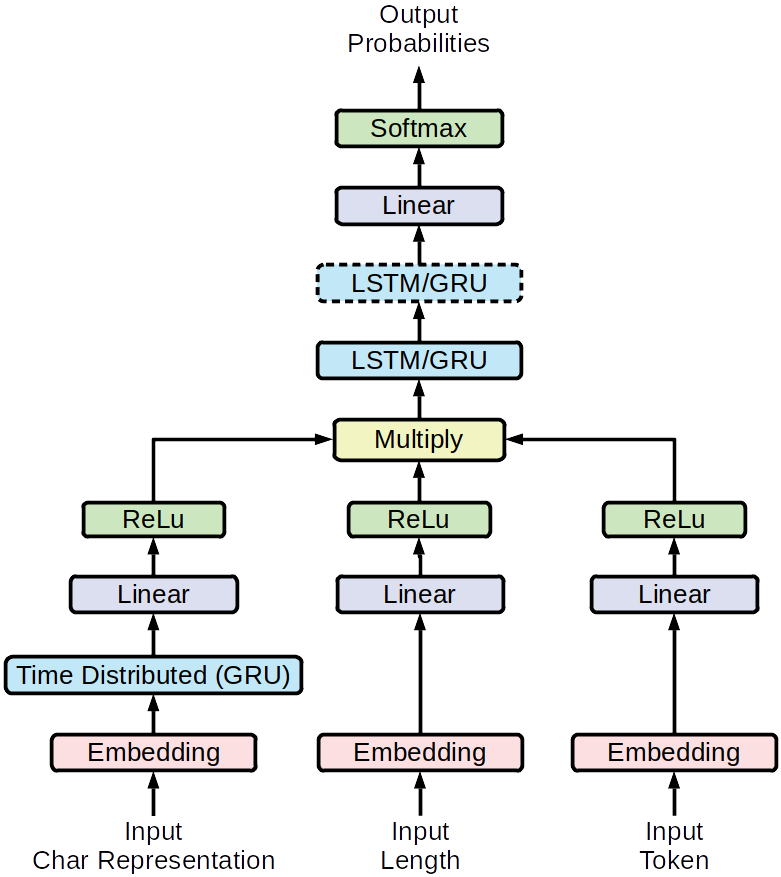
\includegraphics[scale=0.65]{images/model-2.png}%
    \caption{Token, Length \& Char-Processing RNN Architecture}%
    \label{complex-rnn}
\end{figure}

Thus, the final model is made of these three inputs, each of which is separately processed and whose results gets merged into a single vector of a given dimension, which is eventually fed to one or two recurrent layers and a final dense layer with softmax activation, exactly like the previous model.

\subsubsection{\textsc{Hyperparameters and Results}}

Again, here we had the same set of independent hyperparameters for both the variations of the models.
Still, differently from the previous architecture, this one had a larger number of them due to the higher number of inputs, namely:
\begin{itemize}
    \item The dimensions of the \textsc{Token Embedding} layer, the \textsc{Length Embedding} layer and the \textsc{Char Embedding} layer
    \item The dimension of the latent space prior to the \textsc{Multiply} layer 
    \item The kind of \textsc{RNN} (\textsc{GRU} or \textsc{LSTM})
    \item The number of \textsc{RNN} layers (either one or two), and their respective number of units
    \item The dropout rate of the \textsc{RNN} layers
\end{itemize}

After all the tests, this architecture showed scores similar to those of the previous architecture related to the \textit{Subword-Level} variation.
Instead, a slight increase could be noticed on the scores related to the \textit{Word-Level} variation, which were still a little worse than those of the \textit{Subword-Level}.

Given all of this, we decided not to investigate these basic models anymore and try some more recent kinds of architecture.

\section{Verse-Space Seq2Seq RNN}

One of the possible causes of failure encountered in the previous models could be related to the way the original text was partitioned.
In fact, up to the last networks, we developed them to predict one single token given a fixed-length sample of the previous ones, meaning that in the majority of cases we were trying to predict a token in the middle of a verse (thus, having very little information about the rhyming scheme) from a sample starting from a random position inside another verse.
Also, as we generally used a \texttt{step length} grater than one in order both to reduce the computational cost and to avoid overfitting, some of the markers and the tokens at the end of the verse (i.e. those being more useful to understand both the structure and the rhyming scheme) were not used neither for training nor for validating, going "wasted".

\begin{figure}[!htb]
    \centering
    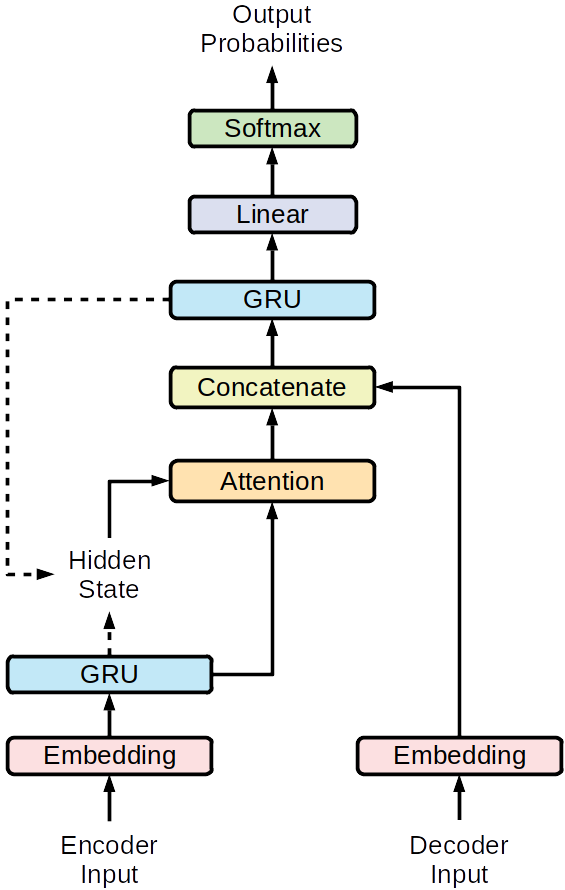
\includegraphics[scale=0.65]{images/model-3.png}%
    \caption{Seq2Seq RNN Architecture}%
    \label{seq2seq}
\end{figure}

Therefore, with the aim of overcoming this structural problem, we tried to use a \textit{Sequence To Sequence} model for \textit{Neural Machine Translation}, also involving attention mechanisms because of the great complexity of the text.
Even though these kind of models are generally used to translate from one natural language to another, we wanted to apply the same idea to the \textit{Divine Comedy}, trying to "translate" a sample of verses into the entire, following verse, and we decided to fix the number of verses, i.e. our new \texttt{sequence lenght}, to three, as from the previous three verses (included the one having as a single token the \texttt{=tercet=} marker) the network should be able to understand both the structure and the rhyming scheme, namely it should be able to understand whether the next verse should contain a \texttt{=tercet=} marker or not, and if not how to properly end the verse so that it rhymes when necessary.

An important thing to be noticed is that, given that the verse to be predicted is the $i_{th}$ one and the input patch is made up of the verses $i-3$ to $i-1$, initially we used as output sequence the output verse only (or rather, the $i_{th}$ verse).
This, however, gave terrible results, in line with the fact that, as well as previous architectures, the network could not understand the inner patterns of the text.
Taking that in mind, we decided at first to use as output a sample of the last three verses (from the $i-2_{th}$ to the $i_{th}$) and, finally, to use all of the four verses as output, because even though the two ways gave almost similar results, in this last case it was easier to perform the prediction/generation phase, as the input sequence had to be entirely passed both to the encoder and to the decoder in order to get as output the last verse only.

Finally, as it can be seen from the picture \ref{seq2seq}, this model is composed of two different, interconnected modules, that are:
\begin{itemize}
    \item an \texttt{\textsc{Encoder}}, made up of an \textsc{Embedding} and a \textsc{GRU} layer, which takes the input sample and returns both the output and the hidden state of the \textsc{GRU}
    \item a \texttt{\textsc{Decoder}}, made up of an \textsc{Embedding} and a \textsc{GRU} layer as well as an \textsc{Attention} layer, which takes the latest decoded token as input, the latest hidden state\footnote{
        During the first iteration, these are the \textit{start token} and the hidden state of the encoder.
    } and the output of the encoder, and returns the hidden state of the \textsc{GRU} and the output processed through a \textsc{Dense} layer
\end{itemize}

As the output returned from this architecture is the vector of probabilities for a single token, we had to develop a custom training loop that repeatedly called the model using the new output (and the new hidden state as well) as inputs until the \textit{end token} of the output sequence was predicted.
This, clearly, led to a more costly training.

\subsubsection{\textsc{Hyperparameters and Results}}

This time, the hyperparameters were:
\begin{itemize}
    \item the dimension of the \textsc{Embedding} layer
    \item the number of units of the \textsc{GRU} layer
    \item the kind of \textsc{Attention} layer, which could be either:
    \begin{itemize}
        \item Additive, or \textit{Bahdanau-style} \parencite{bahdanau2014neural}
        \item Multiplicative, or \textit{Luong-style} \parencite{luong2015effective}
    \end{itemize}
    \item the dropout rate for the \textsc{RNN} layers
\end{itemize}

The main problem of both the variations (\textit{Word-Level} and \textit{Subword-Level}) of this architecture is that, as we said, the training cost was too expensive, with some configuration needing up to twenty minutes per epoch.
This, combined with the fact that the convergence was really slow (looking at the loss/accuracy plots, we saw that the trend was clearly increasing in performances without reaching a plateau, but still this increase was linear and very slight), did not allow us to get great results.
Indeed, the few configurations that were able to achieve results which were greater than the previous two models, did not score well in the \texttt{ngrams plagiarism test}, as they were in fact copying the original verses from the \textit{Divine Comedy}, therefore we decided to abandon the idea of using \textit{RNNs} and exploit, instead, new \textit{state-of-the-art} models for \textit{Neural Machine Translation}. 

\section{Plain Transformer}

The \textit{Transformer} \cite{vaswani2017attention} is a \textit{state-of-the-art} architecture proposed by Vaswani et al.
in 2017 in order to overcome the problems encountered by \textit{RNNs} for \textit{Neural Machine Translation} tasks, namely the poor capacities in long-term memory and attention, and the high computational cost.

\begin{figure}[!htb]
    \centering
    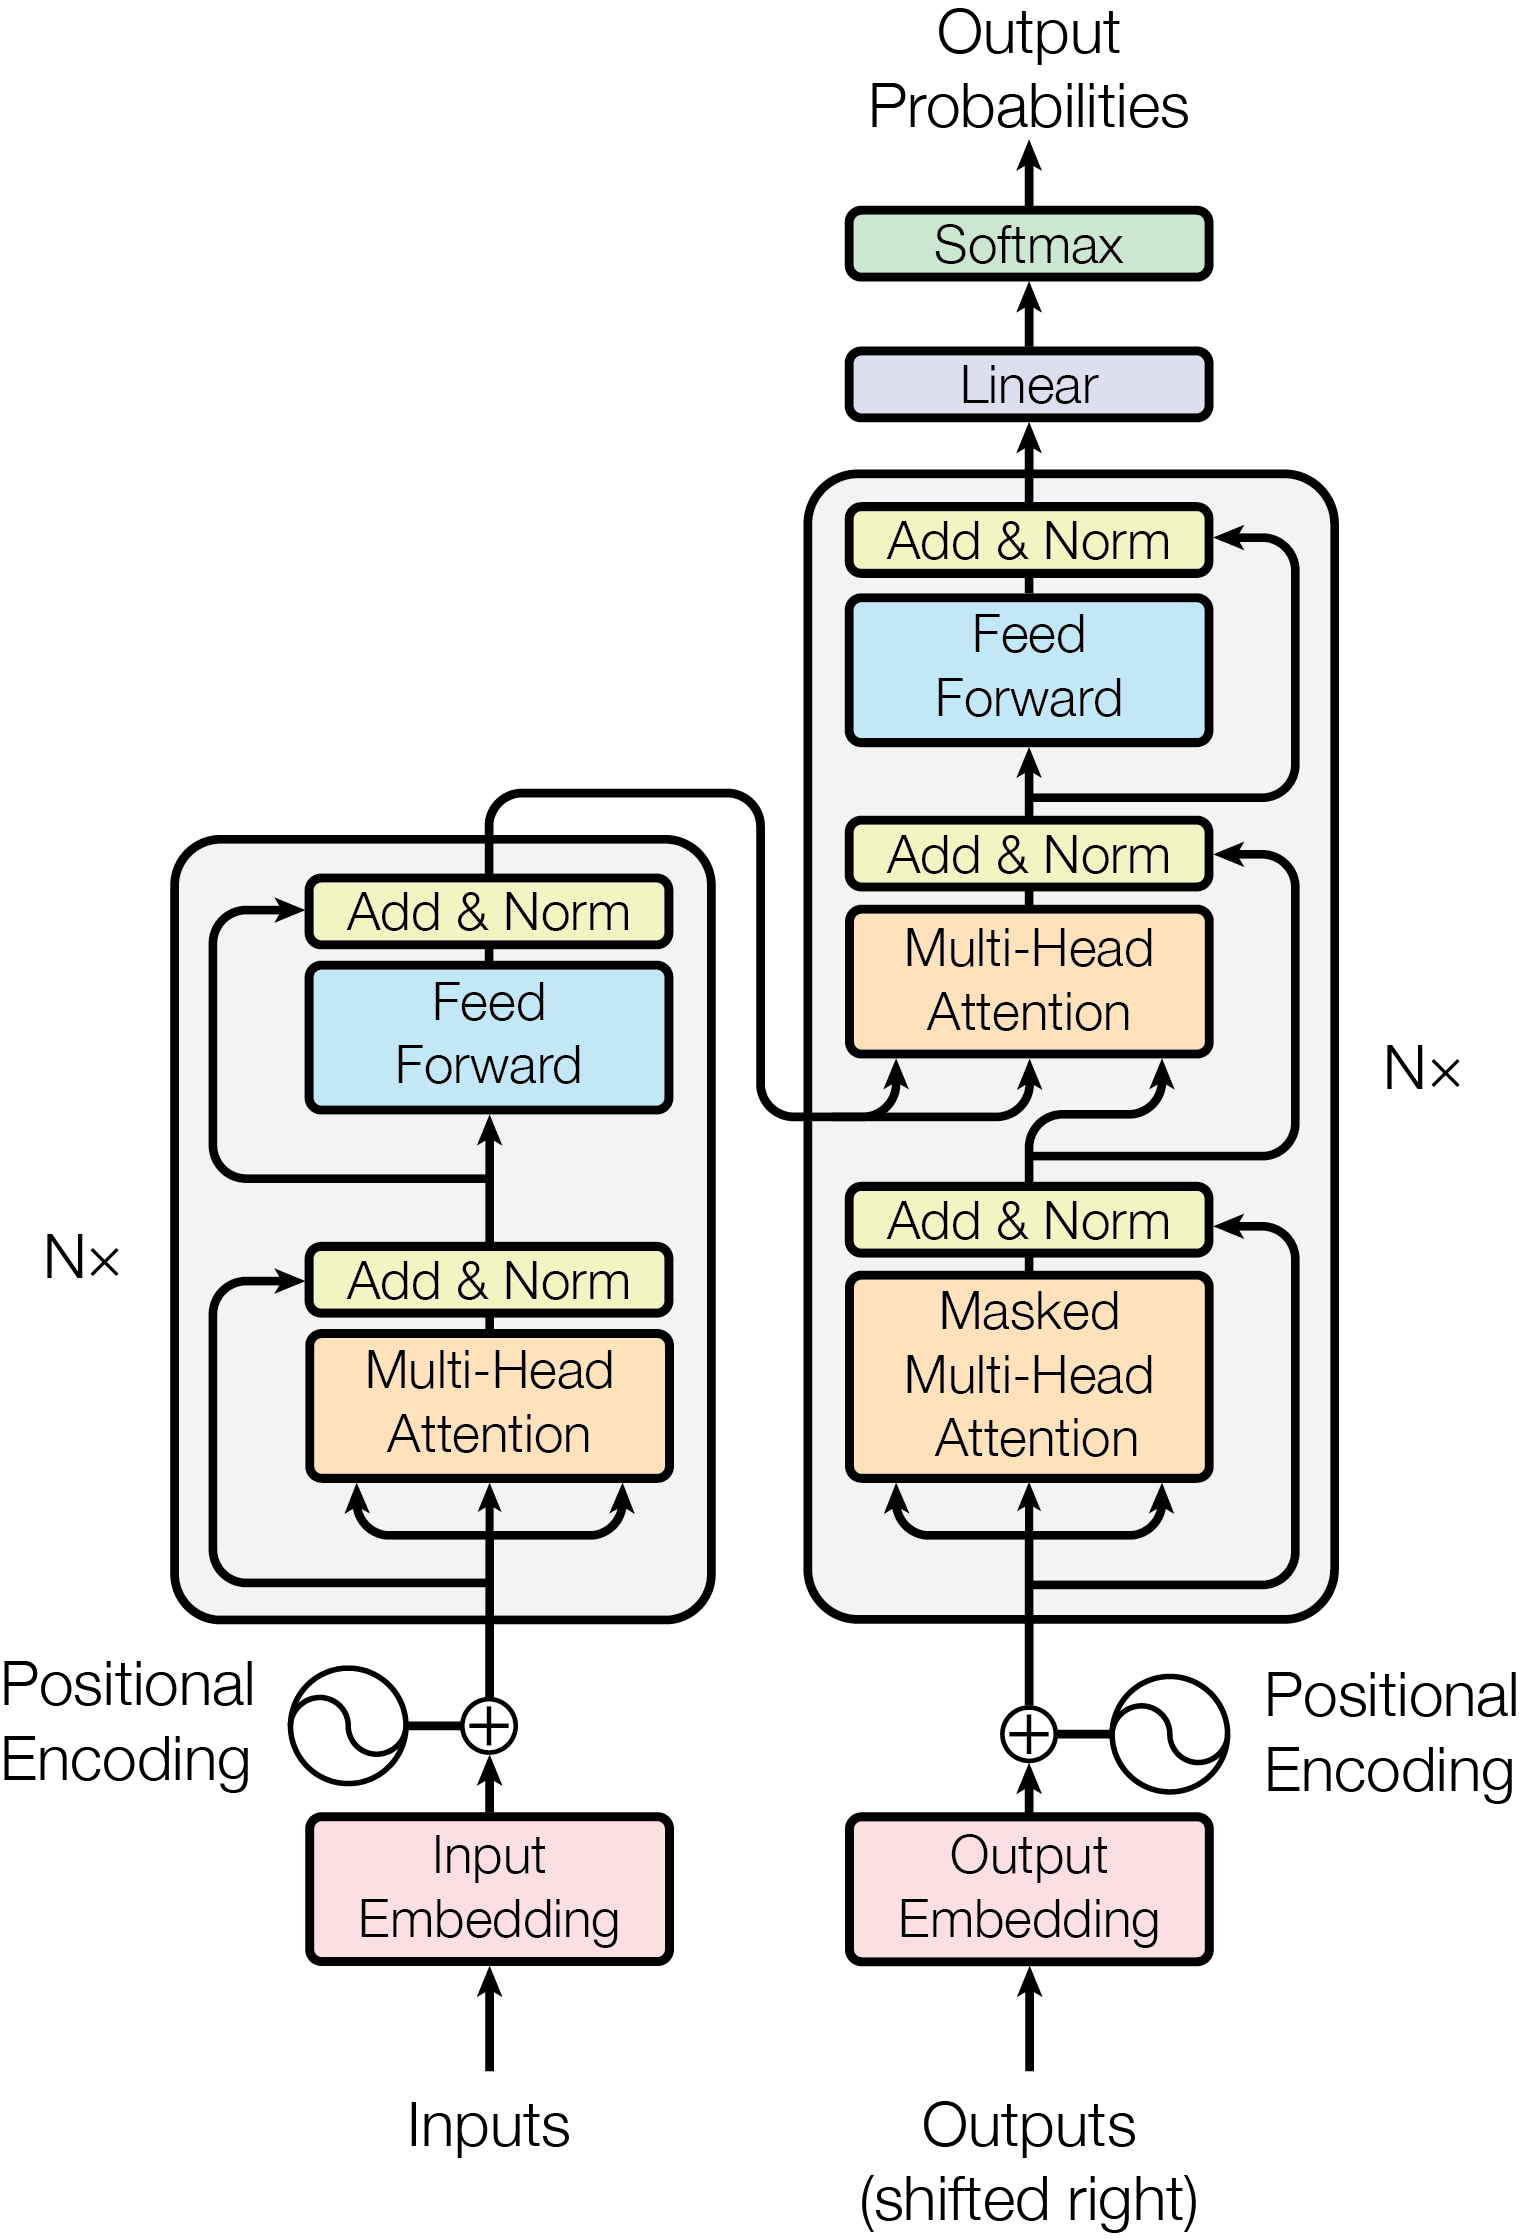
\includegraphics[scale=0.75]{images/model-4_5.png}%
    \caption{Transformer Architecture}%
    \label{transformer}
\end{figure}

As well as standard \textit{Seq2Seq} architectures, the \textit{Transformer} consists of an \texttt{\textsc{Encoder}} and a \texttt{\textsc{Decoder}}, as described in figure \ref{transformer}, both having a number of layers that can be changed in order to have a greater or lower complexity.
Still, differently from previous models, this new one cannot be classified as a recurrent network but it is, instead, a standard feed-forward one, reason why both the \texttt{\textsc{Encoder}}'s and the \texttt{\textsc{Decoder}}'s input tokens must be processed not only with a classical \textsc{Embedding} layer but also with a so-called \textsc{Positional Encoding}, so that the information about the order of the tokens in the sequence is not forgotten even without the presence of recurrent edges.
Finally, these processed inputs are passed through the series of layers, which are made up of two different sub-modules: a \textsc{Multi-Head Attention} (two in the case of the \texttt{\textsc{Decoder}}, as the first one is responsible of processing the decoder input, while the second one is responsible of processing the merged vectors of features extracted both from the encoder input and the decoder input), and a subsequent \textsc{Feed-Forward} block.
Everything is eventually passed through a \textsc{Dense} layer, with softmax activation, to get the output probabilities of each possible token.

The reason why we decided to try this architecture is due to its great ability to generalize in different \textit{Natural Language Processing} tasks as well as its remarkable training speed (being not an \textit{RNN}, it does not suffer the heaviness of backpropagation-through-time).
Furthermore, as we did for the previous models, we decided to start with a simpler version, thus we went back to the standard way of splitting the original text, i.e. with samples of fixed input length and fixed output length, where the output is shifted by one token with respect to the input.

\subsubsection{\textsc{Hyperparameters and Results}}

Though being quite a complex model, the \textit{Transformer} does not have a high number of hyperparameters, which are:
\begin{itemize}
    \item the number of layers for the \texttt{\textsc{Encoder}} and the \texttt{\textsc{Decoder}}
    \item the number of heads for the \textsc{Multi-Head Attention} sub-module
    \item the dimension of all the sub-layers in the model, as well as the \textsc{Embedding} layers, known as \texttt{d\_model}
    \item the inner \textsc{Feed-Forward} layers dimension, known as \texttt{dff}
    \item the dropout rate
\end{itemize}

Overall, this architecture showed a great ability to understand the general structure of the text, as well as our first two models, but in the end nothing more than that could be achieved.
In fact, we could notice a slight increase in the metric for the rhyming scheme, reaching a peak of \textit{0.41} for the \textit{Word-Level} model and \textit{0.44} for the \textit{Subword-Level}, while the score for \texttt{hendecasyllabicness} remained stable for the \textit{Word-Level} and slightly decreased down to a peak of \textit{0.90} for the \textit{Subword-Level} model.

\section{Verse-Space Transformer}

Given that the \textit{Plain Transformer} model gave slightly better results in terms of rhyming scheme, we tried to use the same architecture to perform a more straight-forward \textit{Sequence To Sequence} approach, like we had done for the third model.
Thus, we split again the \textit{Divine Comedy} in single verses and used as input a patch made up of three consecutive verses and, as output, not just the fourth one but the entire patch made up of the all four, exactly as we did for the \textit{Seq2Seq RNN} architecture\footnote{
    Actually, we also tried some configurations in which we used either four or six verses as input, and five or seven as output respectively, but we could not get greater results, probably due to the greater length of the sequences.
}.

\subsubsection{\textsc{Hyperparameters and Results}}

Here, the hyperparameters we had to tune were the same ones of the previous model, i.e. the number of layers, the number of heads, the \texttt{d\_model}, the \texttt{dff} and the dropout rate.

Way more than previous architectures, this one seemed to be very sensible to the variation of the hyperparameters, producing samples having a wider range of scores in the employed metrics.

Also, quite interestingly, tinier models seemed to be more capable of generating better samples.
We interpreted this fact as a proof that, for generative tasks, sometimes it could be better to have a small network which is unable to reproduce the training samples (e.g. in our case, the Neural Network is unable to reproduce the exact \textit{Divine Comedy}) but, instead, it is able to generate samples that, far from being equal, are similar to the training samples.
Instead, this is something that turns out to be almost useless for \textit{Neural Machine Translation} tasks, in which we may need a bigger network with a great ability to reproduce original samples (e.g. to correctly translate a sentence from Italian to English), nevertheless failing at finding more "particular" patterns and, therefore, which would not be able to generate good samples when using higher temperatures during the generative phase.

In the end, even though the \textit{Word-Level} model could not obtain scores that overcame the previous ones (instead, the scores related to the rhyming scheme were lower with respect to almost all of them), maybe due to the fact that we could not find a correct configuration of hyperparameters; the \textit{Subword-Level} model definitely exceeded the bounds set by previous models in terms of rhyming scheme, reaching peaks of \textit{0.89} for that score.
Furthermore, as regards the overall structure of the tercets, the score was optimal for almost all of the tested configurations, while for the \texttt{hendecasyllabicness} we could reach a peak of \textit{0.90} only.
This, though being slightly lower with respect to that of the first two models, can be still considered a good result; in fact, we should take in mind that the provided code used for evaluation, when tested on the first canto of the \textit{Divine Comedy}, due to the complex phenomena of synalephe and dialepha widely used by Dante, did not gave a full score for that particular metric, but returned instead a value which was around \textit{0.94}.

\section{Transformer GAN}

Even though with our last model we could be able to achieve good results in terms of metric scores, we wanted to develop at least one adversarial model \cite{goodfellow2014generative} in order to try getting rid of the \texttt{categorical crossentropy} loss function, which could not always be a good choice for the particular task we were intended to solve.

\begin{figure}[!htb]
    \centering
    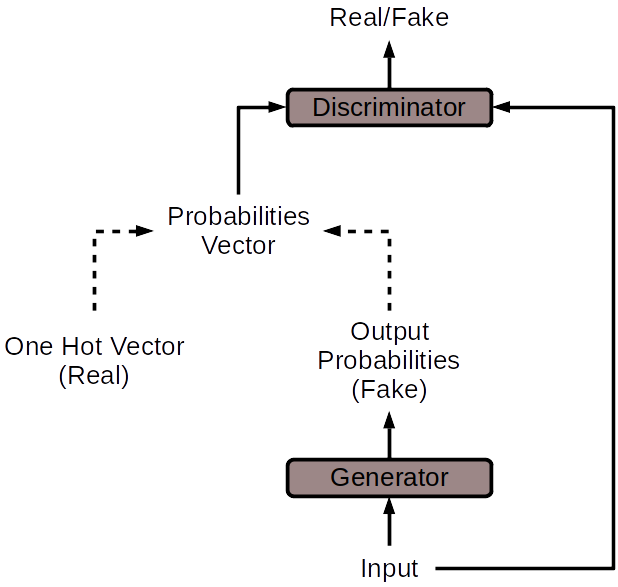
\includegraphics[scale=0.65]{images/model-6-general.png}%
    \caption{Overall GAN Architecture}%
    \label{gan-general}
\end{figure}

Overall, our architecture, as depicted in figure \ref{gan-general}, is composed of a \texttt{\textsc{Generator}} and a \texttt{\textsc{Discriminator}}.
The former takes as input a fixed-length sample of the \textit{Divine Comedy}, as well as the standard \textit{RNN} models and the first version of the \textit{Transformer}, while returning as output a vector of probabilities for the next sample.
Instead, the latter is a \textit{Siamese Network} taking as input both that sample and either the output probabilities vector of the \texttt{\textsc{Generator}} or the one-hot encoded vector representing the actual token.
A closer look of the two modules is presented in the figure \ref{gan-specific}.

\begin{figure}[!htb]
    \centering
    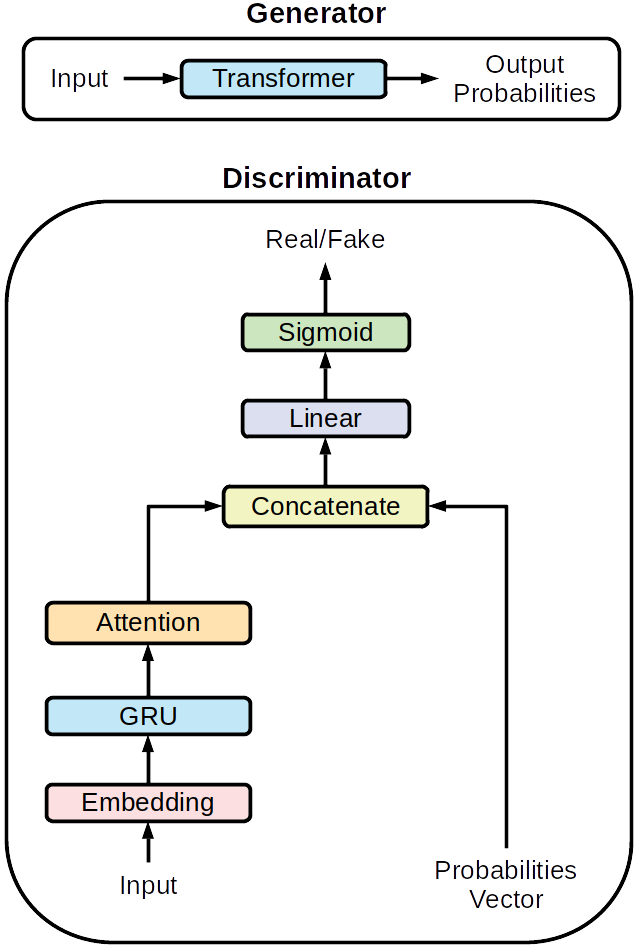
\includegraphics[scale=0.6]{images/model-6-specific.png}%
    \caption{Generator \& Discriminator of the GAN Architecture}%
    \label{gan-specific}
\end{figure}

The reason why we had to switch back to the previous way of splitting the text instead of going on with the verse-level division is that, during the training, it was not possible to generate an entire verse (made up of multiple tokens) at once without having to apply an \textit{hardmax} activation to the generated vectors.
Thus, being the \textit{hardmax} activation non-linear, this would have made impossible to get the gradients related to the weights of the net and, subsequently, to correctly perform the backpropagation step.

\subsubsection{\textsc{Hyperparameters and Results}}

Both the \texttt{\textsc{Generator}} and the \texttt{\textsc{Siamese Discriminator}} had their own hyperparameters to be set.
In particular, those of the \texttt{\textsc{Generator}} are:
\begin{itemize}
    \item the number of layers of the \textit{Transformer}
    \item the number of heads  of the \textit{Transformer}
    \item the dimensions of the latent spaces (\texttt{d\_model} and \texttt{dff})
    \item the dropout
\end{itemize}
while, those of the \texttt{\textsc{Discriminator}} are:
\begin{itemize}
    \item the \textsc{Embedding} dimension
    \item the number of \textsc{GRU} units
    \item the \textsc{Attention} kind
    \item the \textsc{GRU} dropout
\end{itemize}

Even though we tried some different kind of settings, we could never reach the \textit{Nash Equilibrium} between the two modules of the \textit{GAN}\footnote{
    Generally, the \texttt{\textsc{Generator}} seemed to be more powerful than the \texttt{\textsc{Discriminator}}, even for those cases in which we largely reduced its size.
}, which prevented us from having any fit sample at all.

Given that finding an equilibrium during an adversarial train is a well-known complex problem in the field of \textit{Deep Learning}, and that the methods to overcome it require a deep knowledge of many \textit{state-of-the-art} techniques, we decided to stop our investigations here, also given that the results of our previous model were good enough in our opinion.
Anyhow, we shall at least briefly present some of these techniques in the next chapter.